% !TeX root = ../main.tex
% Add the above to each chapter to make compiling the PDF easier in some editors.

\chapter{Compilation in \ac{NAQC}}\label{chapter:compilation}
Compilation is a process of translating a high-level, 
abstract description of a quantum algorithm into a low-level representation of operations suitable for hardware execution.
To do this, this problem divided into multiple subproblems, 
employing different layers of software each for specific subproblems, so-called compilation toolchain.
Moreover, compilation should be familiar with computational capabilities of target hardware.
As described in \ref{chapter:neutralatom} each compilation step for \ac{NAQC} should consider futher hardware constraints.

For example, that together with or instead of SWAP based losing of connectivity problem
there is also possible to shuttle qubit physical, 
compiler should be able to calculate which way will be the most efficient in terms of speed, fidelity, calculation time in the specific situation.

Hence, compiler should consider different execution times of gates, their fidelities, 
and also an available set of gates on current machine.

Moreover, compiler should consider idle time of qubits and calculate corresponding impact from coherence time.
Thus, it should now which operations could be executed parallel and what properties do \ac{AOD} and \ac{SLM} have.

Also, compiler should consider different interaction radius and Rydberg blockade radius, 
and schedule next step according to constraints that go from previous steps and architecture, 
to improve overall quality of compilation.
\parencite{Tan_2025_Enola,Schmid_2024_NeutralAtomBasics}

\section{Compilation Steps}
Consider \ref{fig:compilation_steps}.
\begin{figure}[htbp]
  \centering
    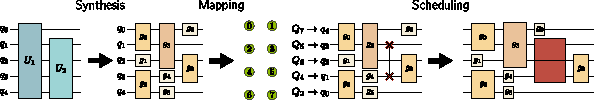
\includegraphics[width=0.8\textwidth]{figures/compilation_steps.pdf}
    \caption[Illustration of the three steps for platform-dependent compilation]{\textbf{Illustration of the three steps for platform-dependent compilation.} In the \textbf{synthesis} step, general operations and unitaries are decomposed into the native gate set $\Sigma_{\mathrm{native}}$.
  During the \textbf{mapping} step, the circuit qubits $q_{i}$ are assigned to physical hardware qubits $Q_{i}$, and necessary SWAP or MOVE operations are introduced to satisfy connectivity constraints.
  Finally, in the \textbf{scheduling} step, gate times and restrictions on parallelism are considered.
  In practice, these steps are often performed simultaneously as a single step rather than sequentially. \parencite{Schmid_2024_NeutralAtomBasics}}
    \label{fig:compilation_steps}
\end{figure}

\section{Considered Toolchains}
In this work three Compiling Toolchains for \ac{NAQC} are considered, 
since they all take a QASM circuit as import and are open-source python projects.
This chapter will cover algorithms that are used by these three, 
describe a workflow, what tools each has, and what consider by compilation
And the result of benchmarking will be evaluated in the next chapter.

\subsection{HybridMapper MQT}
HybridMapper, a Tool from \ac{MQT}, stands out from the previous works, 
because it uses a hybrid compilation approach to map a circuit 
and consider together SWAP gate and Shuttling to explore the potential advantage of leveraging gate-based SWAP insertions 
and shuttling-based atom rearrangements.
When other works individually only considered it separately.
In particular, this is only a mapping and scheduling stage of computation, without synthese and optimization steps.
It simply took a QASM circuit and uses only gates that defined with architecture along with their times, and fidelities 
and doesn't optimize circuit or change something in there, it finds places where interacting conditions are violated 
and solves it with logical or physical move. 
In advance, skipping synthese step gives advantages, 
since other considered toolsets always try to transpile input circuit into Pauli Gates and CZ gate, without consideration of possible multi-qubit CZ gates.

The main idea of algorithm is to use two-capability-specific heuristic cost functions, 
which specially made for fast evaluation 
and consider additional architecture information 
such as number of \ac{AOD} or \ac{SLM} traps, distance between them, interaction radius 
to improve parallelism by using commutation rules and look-ahead functionality \parencite{schmid2023hybridcircuitmappingleveraging}.
Consider for accuracy \ref{fig:overview_HybridMapper}.

\begin{figure}[htbp]
  \centering
    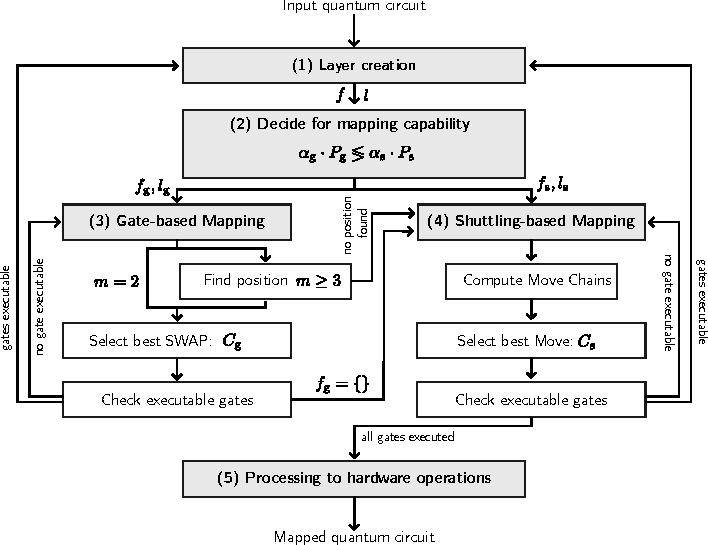
\includegraphics[width=0.8\textwidth]{figures/overviewHybridMapper.pdf}
    \caption{Resulting hybrid mapping process \parencite{schmid2023hybridcircuitmappingleveraging}}
    \label{fig:overview_HybridMapper}
\end{figure}
\subsection{Enola}
Enola a Tool from \ac{UCLA-VAST} based on OLSQ-DPQA uses different approach.
It divides mapping and scheduling steps of compilation into scheduling, placement and routing steps to achieve great fidelity.

Scheduling step is implemented thorough Edge Coloring problem of commutation group (a group consisting of commutable two-qubit
gates that can be executed in any order) graph, 
where vertices are qubits and edges are two-qubit gates. 
This problem then is solved using Misra-Gries algorithm.
For more generic circuits Enola can use the dependency DAG (directed acyclic graph) for the two-qubit
gates in a generic circuit. In this case, the scheduling problem is
straightforward: the optimal number of stages is the critical path
in the DAG and ASAP (as soon as possible) scheduling can achieve
optimality \parencite{Tan_2025_Enola}. Visualization \ref{fig:scheduling_Enola}
\begin{figure}[htbp]
  \centering
    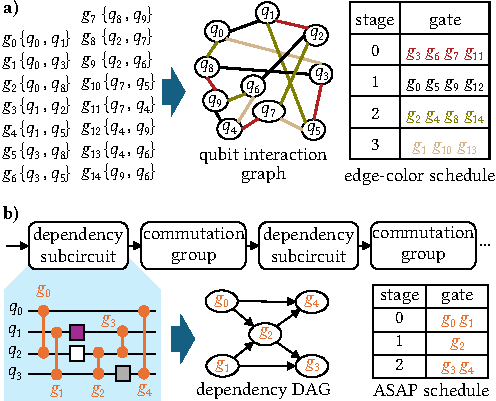
\includegraphics[width=0.8\textwidth]{figures/scheduling_Enola.pdf}
    \caption [Scheduling in Enola]{ Scheduling in Enola. 
    \textbf{(a)} Scheduling a commutation group of two-qubit gates with edge coloring. 
    \textbf{(b)} Generic circuits can be divided to dependency subcircuits and commutation groups. 
    Dependency subcircuits are scheduled ASAP \parencite{Tan_2025_Enola}.}
    \label{fig:scheduling_Enola}
\end{figure}

Placement step is implemented through fast simulated annealing, 
qubits are mapped to interaction sited and the two-qubit
gates at each Rydberg stage are like 2-pin nets in conventional
circuit placement. Hence, the goal is ti minimize total "wire-length".
Fast simulated annealing has three-stages to explore possible states.
At the first stage random search to explore a large solution space is used, the temperature is high, 
thus a high probability of bad solution.
Then, the second stage is a pseudo-greedy local search. 
The last stage is a hill-climbing search where
the temperature increases again to escape from local minima \parencite{Tan_2025_Enola}. 
Visualization \ref{fig:placement_Enola}.
\begin{figure}[htbp]
  \centering
    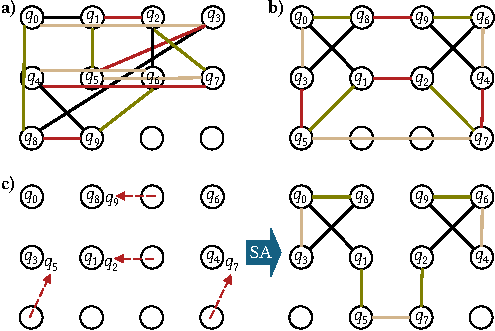
\includegraphics[width=0.8\textwidth]{figures/placement_Enola.pdf}
    \caption[Placement in Enola]{ Placement in Enola. 
    \textbf{(a)} Trivial placement from left to right, from top to bottom. 
    \textbf{(b)} Placement with gate distance optimized by simulated annealing. 
    \textbf{(c)} Dynamic placement: after a Rydberg stage (red) is executed (left), run simulated
    annealing on moved qubits for a new placement (right). \parencite{Tan_2025_Enola}}
    \label{fig:placement_Enola}
\end{figure}

Routing step is used for parallelize \ac{AOD} movements, 
and not to violate fundamental rules of \ac{AOD} such as \textit{the order of its columns cannot change, nor can
the order of rows}.
Then the independent set of vertices is made of possible moves. 
This set will be solved then with maximum independent set solver \parencite{Tan_2025_Enola}.
Visualization \ref{fig:routing_Enola}.
\begin{figure}[htbp]
  \centering
    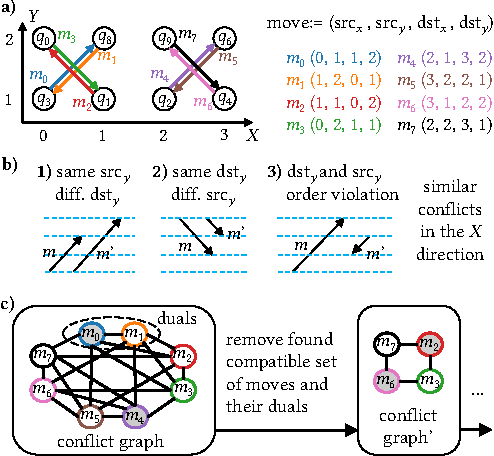
\includegraphics[width=0.8\textwidth]{figures/routing_Enola.pdf}
    \caption[Routing in Enola]{Routing in Enola. 
    \textbf{(a)} Definition of a move as a 4-tuple. 
    \textbf{(b)} Conflicts between two moves. 
    \textbf{(c)} Compatible moves are independent sets (IS) in the conflict graph (filled vertices).
    After finding an IS, delete the moves and their duals from
    the graph. The process continues until no moves are left \parencite{Tan_2025_Enola}.}
    \label{fig:routing_Enola}
\end{figure}

Additionally, Enola always transpiles input circuit into fixed gate set from Pauli Gates and CZ, 
without consideration of a big advantage of \ac{NAQC} that allows to implement different gates.
Also, it considers interaction radius, Rydberg blockade radius, durations and fidelities of gates,
physical placement of \ac{SLM} and \ac{AOD} traps. 
But important note is that Enola doesn't consider number of \ac{AOD}, 
but make an independent set of gates called stages where each pair of gates could be executed without affecting other qubits in that stage.

\subsection{DasAtom}
DasAtom was made as an improvement of Enola and Tetris 
and used the weakest aspects of each to strengthen and made itself.
Enola leverages atom shuttling to adapt qubit mappings dynamically,
but cannot take advantage of long-range interactions
and Tetris' main idea is to leverage the long-range interactions of \ac{NAQC} 
to achieve denser qubit connectivity\parencite{10082942, huang2025dasatomdivideandshuttleatomapproach}.

The main idea of DasAtom is a bit changed \ac{DAC} approach to divide circuit into subcircuits.
It was inspired from different DAC adaptations from \parencite{siraichi:hal-02316820, 10.1145/3508352.3549394, huang2024qubitmappingadaptivedivideandconquer}
Then it assigns an optimal qubit mapping for each subcircuit, and then shuttles
atoms to smoothly transition between mappings. This approach should improve overall fidelity and efficiency.
Consider \ref{fig:DasAtomFlowChart}

\begin{figure}
\centering
\scalebox{0.78}{
\begin{tikzpicture}[node distance=1.5cm]

% Nodes
\node (start) [startstop] {Input: CZ circuit $C$, $d$, $R_{\mathrm{int}}$, $R_{\mathrm{restr}}$};
\node (partition1) [process, below of=start] {Divide $C$ into CZ layers $L_1,...L_m$};
\node (partition2) [process, below of=partition1] {Divide $C$ into $C_1, ..., C_k$ and find an embedding $f_i$ for each $C_i$};
%\node (init) [process, below of=partition2] {Let $i = 1$};
\node (execute) [process, below of=partition2] {Start with $i=1$ and execute $C_i$ with $f_i$};
\node (decision) [decision, below of=execute, yshift=-0.5cm] {$i = k?$};
\node (route) [process, below of=decision, yshift=-0.5cm] {Route $f_i$ to $f_{i+1}$};
\node (increment) [process, left of=route, xshift=-2.5cm] {$i = i + 1$};
\node (end) [startstop, right of=decision, xshift=1.5cm] {End};
% Arrows
\draw [arrow] (start) -- (partition1);
\draw [arrow] (partition1) -- (partition2);
\draw [arrow] (partition2) -- (execute);
\draw [arrow] (execute) -- (decision);
\draw [arrow] (decision) -- node[anchor=east] {no} (route);
\draw [arrow] (route) -- (increment);
\draw [arrow] (increment) |- (execute.west);
\draw [arrow] (decision) -- node[anchor=south] {yes} (end);

\end{tikzpicture}}
\caption{The flowchart of DasAtom \parencite{huang2025dasatomdivideandshuttleatomapproach}.}
\label{fig:DasAtomFlowChart}
\end{figure}

DasAtom states about 415.8 times higher fidelity comparing to Enola in \ac{QFT}30. 
This statement doesn’t quite seem to be full correct.
\parencite{huang2025dasatomdivideandshuttleatomapproach}